\documentclass[a4paper]{article}
\usepackage[14pt]{extsizes} % для того чтобы задать нестандартный 14-ый размер шрифта
\usepackage[utf8]{inputenc}
\usepackage[russian]{babel}
\usepackage{setspace,amsmath}
\usepackage[left=20mm, top=15mm, right=15mm, bottom=15mm, nohead, footskip=10mm]{geometry} % настройки полей документа
\documentclass{article}
\usepackage{graphicx}
\graphicspath{ {images/} }

\begin{document} % начало документа
	
	% НАЧАЛО ТИТУЛЬНОГО ЛИСТА
	\begin{center}
		\hfill \break
		\large{МИНОБРНАУКИ РОССИИ}\\
		\footnotesize{МИНИСТЕРСТВО ОБРАЗОВАНИЯ РОССИЙСКОЙ ФЕДЕРАЦИИ}\\ 
		\footnotesize{НАЦИОНАЛЬНЫЙ ИССЛЕДОВАТЕЛЬСКИЙ УНИВЕРСИТЕТ}\\
		\small{\textbf{«МОСКОВСКИЙ ЭНЕРГЕТИЧЕСКИЙ ИНСТИТУТ»}}\\
		\hfill \break
		\normalsize{Кафедра РМДиПМ}\\
		\hfill \break
		\hfill\break
		\hfill\break
		\hfill \break
		\hfill \break
		\hfill \break
		\normalsize{Курсовая работа}\\
		\normalsize{По курсу «Вычислительная механика» на тему:}\\
		\normalsize{Численное моделирование движения шестизвенного манипулятора при перемещении схвата по заданному закону}\\
		\hfill \break
		\hfill \break
		\hfill \break
		
		\hfill \break
		
		\hfill \break
		\hfill \break
	\end{center}
	\hfill \break
	\hfill \break
	\hfill \break
	
	
	\hfill \break
	\vbox{%
		\hfill%
		\vbox{%
			\hbox{студент Волошанин Д.М.}%
			\hbox{Вариант 2}%
			\hbox{Модель робота Hyundai HX400S}%
			\hbox{группа С-12б-19}%
			\hbox{Преподаватель Адамов Б.И.}%
			\hbox{Работа зачтена: }%
		}%
	} 
	\hfill \break
	\hfill \break
	
	
	\hfill \break
	\hfill \break
	\begin{center} Москва 2022 \end{center}
	\thispagestyle{empty} % выключаем отображение номера для этой страницы
	
	% КОНЕЦ ТИТУЛЬНОГО ЛИСТА
	
	\newpage
	
	\tableofcontents % Вывод содержания
	\newpage
	
	\newpage
	\section{Введение}
	Цель работы: проведение численного моделированная движения шестизвенного
	манипулятора при перемещении схвата по заданному закону.
	\hfill \break
	\hfill \break
	Исходные данные: кинематическая схема промышленного шестизвенного манипулятора Hyundai HX400S. 
	(Вид траектории и закон движения выходного звена зависят от промежуточных
	результатов и будут определены в процессе выполнения работы.)
	\hfill \break
	
	\begin{figure}[h]
		\centering
		\includegraphics[width=0.25\textwidth]{manipul_im}
		\caption{Манипулятор Hyundai HX400S}
		\label{fig:mesh1}
	\end{figure}
	\hfill \break
	\begin{figure}[h]
		\centering
		\includegraphics[width=0.4\textwidth]{obl_deysv_man}
		\caption{Рабочая область манипулятора Hyundai HX400S}
		\label{fig:mesh2}
	\end{figure}
	\hfill \break
	\hfill \break
	\hfill \break
	Этапы решения поставленной задачи:
	\begin{enumerate}
		\item Построить программное движение схвата. Задать траекторию схвата в пределах
		рабочей области манипулятора. Траектория представляет собой замкнутую
		плоскую ломанную, её обход производится с постоянной скоростью и неизменной
		пространственной ориентацией схвата.
		
		\item Определить движение звеньев при отработке программного движения путём
		решения обратной задачи кинематики (численного решения дифференциальных
		уравнений кинематики манипулятора или обратной задачи о положениях)
	\end{enumerate}
	
	
	\newpage
	\section{Часть 1. Описание движения манипулятора с помощью параметров Денавита-Хартенберга. }
	\begin{figure}[h]
		\centering
		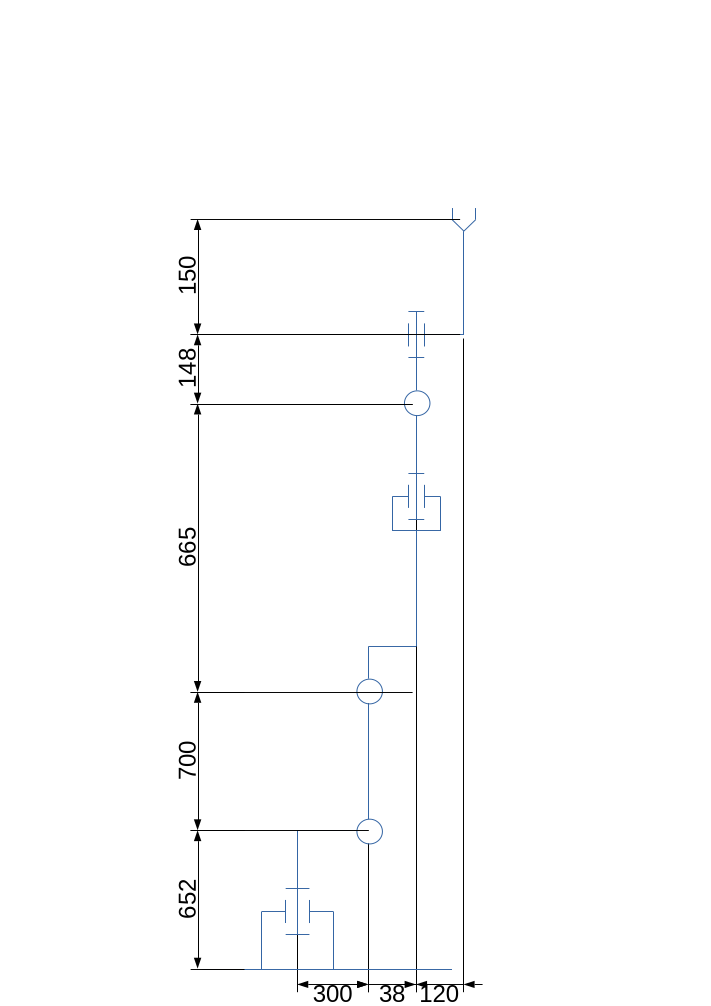
\includegraphics[width=0.5\textwidth]{Курсовая работа_TUR15.png}
		\caption{Кинематическая схема манипулятора Hyundai HX400S}
		\label{fig:mesh3}
	\end{figure}
	Введем систему координат Денавита-Хартенберга.
	\hfill \break
	\hfill \break
	\begin{figure}[h]
		\centering
		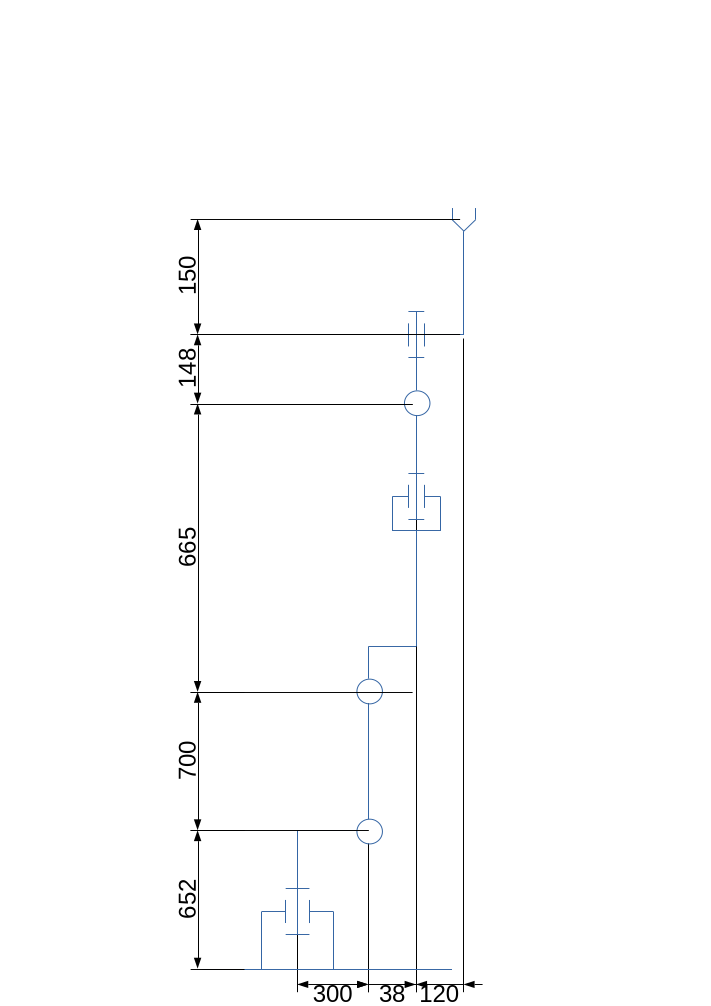
\includegraphics[width=0.78\textwidth]{Курсовая работа_TUR15.png}
		\caption{Кинематическая схема манипулятора Hyundai HX400S}
		\label{fig:mesh3}
	\end{figure}
	\hfill \break
	\hfill \break
	\hfill \break
	Составим таблицу параметров.
	\hfill \break
	\hfill \break
	\centering
	\begin{center}
		\begin{tabular}[c]{l|l|l|l|l|l}
			\textbf{№} & Тип к-с & \Theta_i & d_i & a_i & 	\alpha_i \\[2mm]\hline
			1 & вр & 0°& 1050 &  350 & 90°\\
			2 & вр & 90°& 0 & 1000 & 0° \\
			3 & вр & 0°& 0 & 200 & 90°  \\
			4 & вр & 0°& 1800 & 0 & -90°  \\
			5 & вр & 0°& 0 & 0 & 90°  \\
			6 & вр & 0°& 258 & 0 & 0°  \\
		\end{tabular}
	\end{center}
	\hfill \break
	\hfill \break
	Найдем матрицу преобразований в общем виде
	\hfill \break
	\hfill \break
	\begin{equation}
		T = T_d*T_\Theta*T_a*T_\alpha
	\end{equation}
	\hfill \break
	\hfill \break
	\begin{equation*}
		T =
		\begin{pmatrix}
			1 & 0 & 0 & 0\\
			0 & 1 & 0 & 0\\
			0 & 0 & 1 & d\\
			0 & 0 & 0 & 1
			
		\end{pmatrix}
		*
		\begin{pmatrix}
			cos(\Theta)&  -sin(\Theta)& 0 & 0\\
			sin(\Theta)&   cos(\Theta)& 0 &0 \\
			0& 0 & 0 &0 \\
			0& 0 & 0 & 1
			
		\end{pmatrix}
		*
		\begin{pmatrix}
			1 &  0&  0&a \\
			0 &  1&  0& 0\\
			0& 0 & 1 & 0\\
			0&0  &  0& 1
			
		\end{pmatrix}
		*
		\begin{pmatrix}
			1&  0&  0& 0\\
			0&  cos(\alpha) & sin(\alpha) & 0\\
			0& sin(\alpha) &   cos(\alpha)& 0\\
			0& 0 & 0 & 1
			
		\end{pmatrix}
	\end{equation*}
	\begin{equation*}
		=
		\begin{pmatrix}
			cos(\Theta)&  -sin(\Theta)& 0 & 0\\
			sin(\Theta)&   cos(\Theta)& 0 &0 \\
			0& 0 & 0 &d \\
			0& 0 & 0 & 1
			
		\end{pmatrix}
		*
		\begin{pmatrix}
			1 &  0&  0&a \\
			0 &  1&  0& 0\\
			0& 0 & 1 & 0\\
			0&0  &  0& 1
			
		\end{pmatrix}
		*
		\begin{pmatrix}
			1&  0&  0& 0\\
			0&  cos(\alpha) & sin(\alpha) & 0\\
			0& sin(\alpha) &   cos(\alpha)& 0\\
			0& 0 & 0 & 1
			
		\end{pmatrix}
		= 
	\end{equation*}
	\begin{equation*}
		=
		\begin{pmatrix}
			cos(\Theta)&  -sin(\Theta)& 0 & a*cos(\Theta)\\
			sin(\Theta)&   cos(\Theta)& 0 &a*sin(\Theta) \\
			0& 0 & 0 &d \\
			0& 0 & 0 & 1
			
		\end{pmatrix}
		*
		\begin{pmatrix}
			1&  0&  0& 0\\
			0&  cos(\alpha) & sin(\alpha) & 0\\
			0& sin(\alpha) &   cos(\alpha)& 0\\
			0& 0 & 0 & 1
			
		\end{pmatrix}
		= 
	\end{equation*}
	\begin{equation*}
		=
		\begin{pmatrix}
			cos(\Theta)&  -sin(\Theta)*cos(\alpha)& sin(\Theta)*sin(\alpha) & a*cos(\Theta)\\
			sin(\Theta)&   cos(\Theta)*cos(\alpha)& -cos(\Theta)*sin(\alpha) &a*sin(\Theta) \\
			0& 0 & cos(\alpha) &d \\
			0& 0 & 0 & 1
			
		\end{pmatrix}
		
	\end{equation*}
	
	Построим рабочую область манипулятора (без учета самопересечений) с использованием Wolfram Mathematica
	\hfill \break
	\hfill \break
	\hfill \break
	\hfill \break
	Для этого необходимо перевести допустимые табличные значения углов в допустимые значения углов \Theta
	\hfill \break
	\hfill \break
	\begin{center}
		\begin{tabular}[c]{l|l|l|l|l|l}
			\textbf{№ шарнира} & Табличное значение & \ смещение & \Theta_i \\[2mm]\hline
			1 & -180°... 180° & 0°& -180°... 180°\\
			2 & -50°... 95° & 90°& 0 45°... 185° \\
			3 & -25°... 120° & 0°& -25°... 120°  \\
			4 & -360°... 360° & 0°& -360°... 360°  \\
			5 & -120°... 120° & 0°& -120°... 120° \\
			6 & -360°... 360° & 0°& -360°... 360° \\
		\end{tabular}
	\end{center}
	\newpage
	\section{Часть 2. Построение рабочей области манипулятора в вертикальной плоскости.}
	
	\newpage
	\section{Часть 3. Определение законов изменения обобщённых координат на программном
		движении.}
	
	\newpage
	\section{Часть 4. Определение законов изменения обобщённых координат на программном
		движении.}
\end{document}  % КОНЕЦ ДОКУМЕНТА !